\documentclass[main.tex]{subfiles}

\begin{document}
\section{Modelli di classificazione}
I modelli utilizzati per classificare sono: l'analisi discriminante lineare (LDA) e quadratica (QDA), il modello multinomiale e l'albero di classificazione. In tabella~\ref{tab:acc} sono riportate le percentuali di accuratezza per ogni modello valutate sull'insieme di convalida.
\begin{table}[H]
\centering
\caption{Accuratezza per i modelli adattati.}
\begin{tabular}{cc}
\toprule
       Modello &  Accuratezza \% \\
\midrule
 Multinomiale &          85.87 \\
           QDA &          85.87 \\
 Decision Tree &          82.94 \\
           LDA &          72.66 \\
\bottomrule
\end{tabular}
\label{tab:acc}
\end{table}

La classificazione migliore è ottenuta con il modello multinomiale, la cui matrice di confusione è riportata in Figura~\ref{fig:mn}.
\begin{figure}[H]
	\centering
	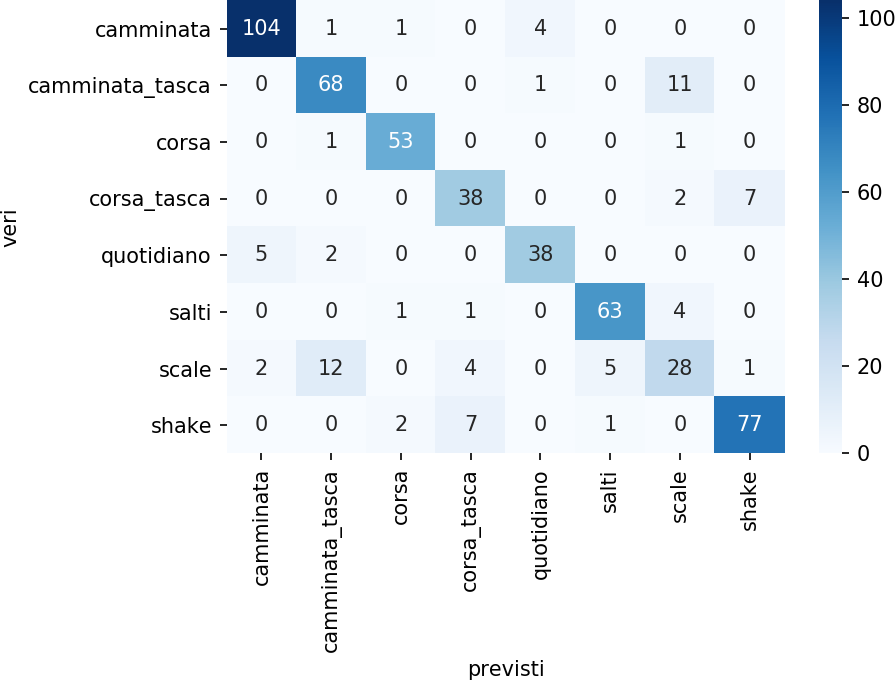
\includegraphics[width=\confusion]{../../figure/confusionMatrix-Mn.png}
	\caption{Matrice di confusione ottenuta con il modello multinomiale.}
	\label{fig:mn}
\end{figure}

Si può valutare l'importanza delle variabili esplicative tramite l'albero di classificazione ottimizzato (Figura~\ref{fig:importance-Tree}), calcolando la riduzione media dell'impurità di Gini data dalla variabile \cite{DecisionTreeClassifier}.
\begin{figure}[H]
	\centering
	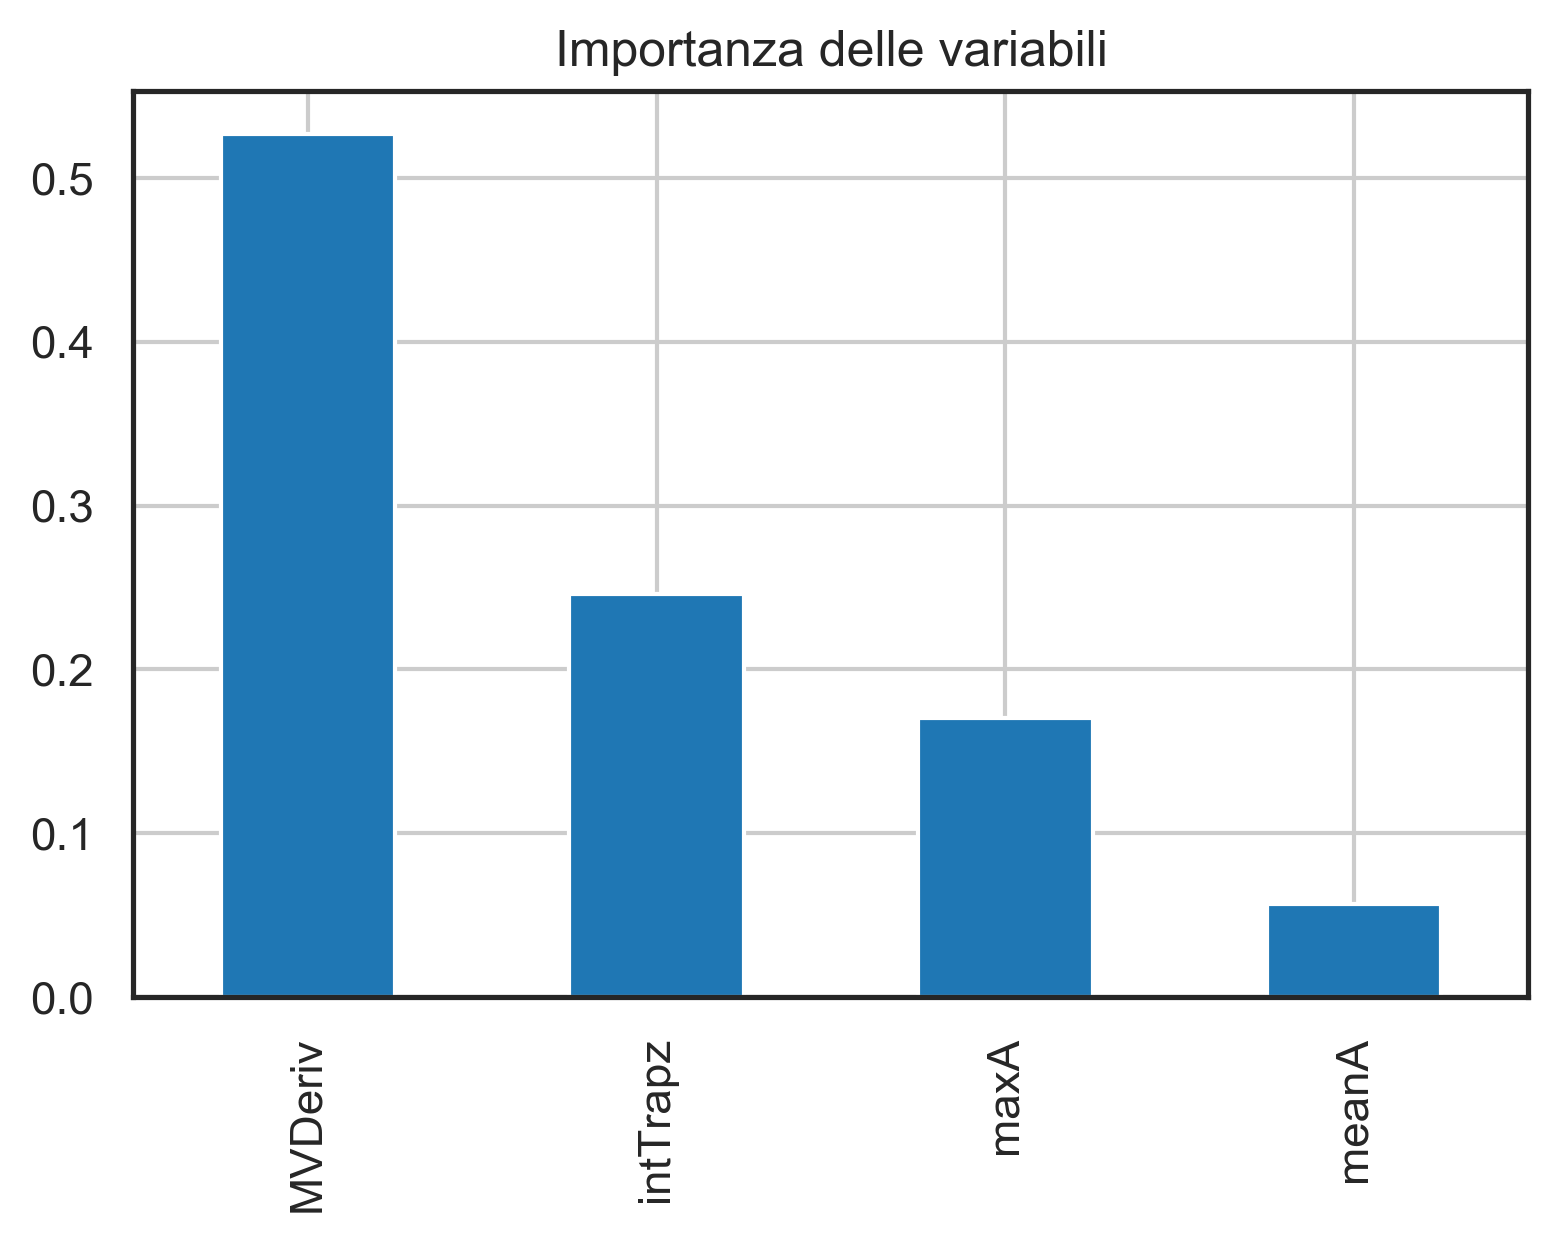
\includegraphics[width=0.82\confusion]{../../figure/importance-Tree.png}
	\caption{Importanza delle variabili ottenuta con l'albero di classificazione.}
	\label{fig:importance-Tree}
\end{figure}
La variabile più rilevante per l'albero risulta essere \texttt{MVDeriv}, confermando quanto ipotizzato nel preprocessamento. Il massimo e il minimo dell'accelerazione sono, invece, le variabili meno importanti: non eliminando l'effetto dell'accelerazione di gravità, esse sono molto dipendenti dall'orientazione del cellulare durante il movimento.
\end{document}